% \section{Double Descent from an Implicit Label Noise Perspective}
% \section{Adversarial perturbation can cause label noise implicitly}
% \section{Explore Label Noise in Adversarial Training}
% \label{sect:reason}

% \chengyu{Make sure we show the point that adversarial training only \emph{magnifies} the label noise and thus makes the robust overfitting more evident.}

% \chengyu{Avoid mention double descent to the best}

% \chengyu{maybe also no need to define ``implicit label noise''. Then people will not require us to demonstrate such a new type of label noise in the reality.}

% In this section, we present a novel perspective to understand the double descent in adversarial training. The implicit label noise is originated from the improper labeling of the adversarial examples and can induce double descent in adversarial training.

% In this section, we first show that traditional adversarial perturbation does not cause label noise directly. We then argue that adversarial perturbation cause label noise implicitly, but significantly.

% To understand intriguing behaviors of adversarial training such as robust overfitting we focus on its training set. We first show that label noise does not explicitly exist in the adversarially augmented training set. We then argue that label noise will implicitly exist in the adversarially augmented training set due to the distribution mismatch and improper label construction in the common practice.


 




% % ----------------------------------------------
% ----------------------------------------------
% \subsection{Traditional adversarial label \textbf{does not introduce label flipping noise}}
% \subsection{Traditional adversarial label does not introduce label noise directly}
\subsection{Label noise does not explicitly exist in the adversarially augmented training set}
\label{sect:label-flipping-noise}

\chengyu{Remove this section?}
% \sout{In standard learning, it is often necessary to manually inject label noise to make the double descent evident for modern neural architectures~\citep{Nakkiran2020DeepDD, Yang2020RethinkingBT}.}

% Since label noise is often essential to explain double descent in standard learning for modern neural architectures~\citep{Nakkiran2020DeepDD, Yang2020RethinkingBT},
% We wish to check if the traditional adversarial label produces any label flipping noise, a typical type of label noise, namely if $\tilde{y}_\delta \ne y^*_\delta$ for any adversarial example $x_\delta$.
% \chengyu{It is still possible there is a tiny fraction of label noise. But won't make a big difference.}
% the assigned label of the adversarial example is different from its true label.
% This is equivalent to checking if $ y^* \ne y_\delta^* $, since $\tilde{y}_\delta = y$ by the definition of the traditional adversarial label (Definition~\ref{remark:common-practice}) and $y = y^*$ by the property of our clean dataset (Assumption~\ref{assumption:clean-dataset}). Note that $y^* \ne y_\delta^*$ means the semantics of the adversarial example is distorted significantly such that its argmax label is now different from the argmax label of its clean counterpart. % , which is possible under adversarial perturbation.


    % The common practice in adversarial training assumes that an adversarial example shares the same true label with its clean counterpart, i.e., $\hat{y}_{\delta} \leftarrow \hat{y}$.
    % Since we have to pick one label for each instance and we have assumed $p(\hat{y} | x) = p(y | x)$, this assumption can be formally viewed as ``$\argmax_j ~p(y_{\delta}=j|x + \delta) = \argmax_j ~p(y=j|x)$''. 
    % Here, we show that this assumption does not introduce label flipping noise, which is often necessary to produce double descent in modern neural architectures in standard classifier training.


% \begin{figure*}[!ht]
% \centering
% % \begin{subfigure}{1.0\textwidth}
%   \centering
%   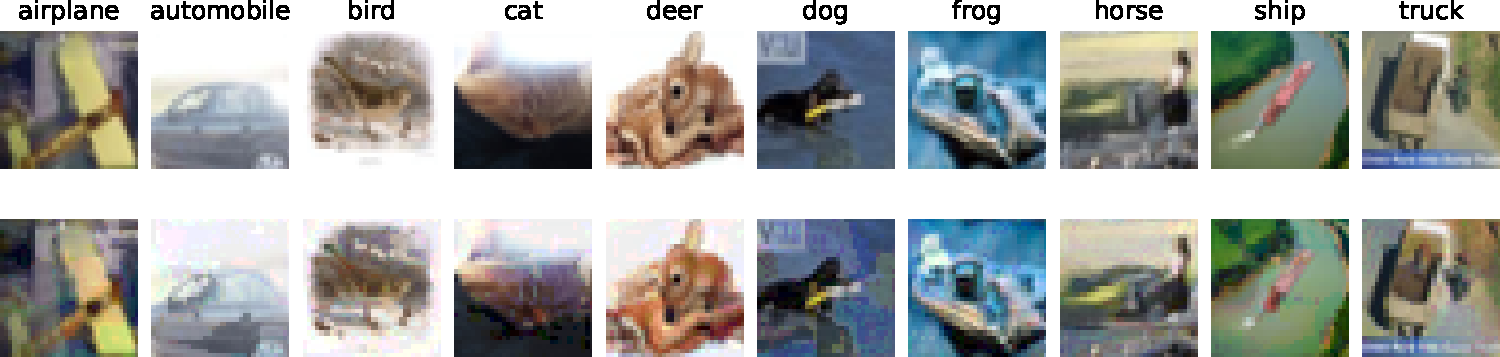
\includegraphics[width=0.95\linewidth]{figures/examples-low-quality.pdf}
%   % \caption{Examples with the lowest quality and their corresponding adversarial examples.}
%   % \label{fig:problematic-examples-orig}
% % \end{subfigure}
% % \begin{subfigure}{1.0\textwidth}
% %   \centering
% %   \includegraphics[width=0.95\linewidth]{figures/examples-high-quality.pdf}
% %   \caption{Examples with the highest quality and their corresponding adversarial examples.}
% %   \label{fig:problematic-examples-ad}
% % \end{subfigure}
%   \caption{Examples with the lowest and highest quality identified in the training set of CIFAR-10. In each subfigure, the top row shows the original image and the bottom row shows the image after the adversarial perturbation (PGD-10 with perturbation radius $8/255$). For each image, the true label is annotated on the top.}
%   % , and the predicted label is annotated on the bottom.}
% \label{fig:examples}
% \end{figure*}



We check if the adversarially augmented training set constructed from the benchmark dataset contains any noisy labels, namely the assigned labels that are different from their corresponding true labels.
    % We first visually check the adversarial examples created by the inner maximization in adversarial training. 
    We are specifically interested in those inputs with the lowest data quality as they are mostly likely to become label noise after perturbation.
    We estimate data quality based on model ensemble (see Appendix~\ref{sect:data-quality-estimation}).
    One can find that the adversarial examples of those low-quality inputs still match their original labels, albeit being slightly more ambiguous (see Figure~\ref{fig:illustration} and \todo{more samples in Appendix.}). 
    
    Evidence can also be found by charting the geometrical structure of the benchmark dataset.
    % \citet{Yang2020ACL} study the distance between examples in the input space. 
    In CIFAR-10 training set, \citet{Yang2020ACL} found that the minimum distance between any two inputs with different labels is around $50/255$ in terms of $\ell_\infty$ norm. In contrast, the perturbation radius used in adversarial training is typically $8/255$, which is significantly smaller. Therefore, it is unlikely that adversarial perturbation will change the true labels of the training inputs.
    It is thus reasonable to argue that label noise does not explicitly exist in the adversarially augmented training set in abundance.
    % Subsequently it cannot adequately explain the double descent observed in adversarial training.

version https://git-lfs.github.com/spec/v1
oid sha256:9956ecf8f72f8cc864de3724da585c24c2cb6e97975537af55723da00e24101f
size 19514


% \subsection{Equivalence between implicit label noise and label flipping noise}
% \subsection{Influence of implicit label noise in adversarial training}
% \subsection{Influence of implicit label noise}
% \subsection{Implicit label noise is a specific type of label noise}
% \smallsection{Connection and difference between implicit label noise and conventional label noise}
\smallsection{Intuitive interpretation of label noise in adversarial training}
% \chengyu{If no section 4.1, can also remove this section}
% In this section, we connect the implicit label noise to a more familiar definition of label noise and show it can have a significant impact.
%     \begin{proposition}[Implicit label noise is equivalent to instance-dependent and class-dependent label noise]
%     \label{proposition:label-noise}
%     Let $p_e(j, x) = P(\tilde{Y}\ne j | Y = j, x)$ be a typical definition of label noise which depends on both the class $j$ and input $x$. Then implicit label noise is equivalent to
%     \begin{equation}
%       % p(Y\ne Y^* | x) = 1 - \sum_j p(Y= j | Y^* = j, x) p(Y^* = j|x),
%       P(\tilde{Y}\ne Y | x) = 1 - \sum_j (1 - p_e(j, x)) P(Y = j|x),
%     \end{equation}
%   % It can easily seen that if $p(Y\ne Y^* | x) > 0$, $p(Y\ne j | Y^* = j, x) > 0$ for some $j$.
%   \end{proposition}
%   \begin{proof}
%   See Appendix~\ref{sect:label-noise-more-proof}.
%   \end{proof}
We introduce a simple example to help understand the emergence of label noise in adversarial training.
% Towards an intuitive understanding of implicit label noise, we introduce a simple example to discuss the differences and connections between implicit label noise and convention label noise.
% We now try to quantify the implicit label noise given its connection with typical label noise.
% \chengyu{We now discuss a simplified example of implicit label noise, and discuss its connection and difference with conventional label noise.}
\begin{example}
% [Quantify the implicit label noise]
[Label noise due to a symmetric distribution shift]
\label{example:label-noise-influence}
% We would like to note that the adversarial training setting would amplify the impact of the implicit label noise, since it adds perturbations to every training sample. 
% In fact, Theorem 3.1 in our main paper, which lower-bounds the implicit label noise by the distance between the assigned label distribution and the true label distribution, provides a way to intuitively quantify the implicit label noise. 
Let $\mathcal{D}=\{(x_i, y_i)\}_{i\in[N]}$ be a clean labeled training subset where all inputs $x_i=x$ are identical and have a one-hot true label distribution, i.e., $P(Y|x) = \mathbf{1}_y$. %, and there is no label noise in $\mathcal{D}$, i.e. $y = \tilde{y}$. 

We now construct an adversarially augmented training subset $\mathcal{D'} = \{(x'_i, \tilde{y}'_i)\}_{i\in[N]}$, where $\tilde{y}' = y$ and $x'$ is generated based on adversarial perturbation that distorts the true label distribution symmetrically. Specifically,
$$
P(Y'= j' | x') =
\begin{cases} 
1 - \eta, & \text{if}~~j = y, \\
\eta/(K-1), & \text{otherwise}. \\
\end{cases}
$$
Then by Lemma~\ref{theorem:implicit-label-noise} 
% we have $P(\tilde{Y}' \ne Y' | x') \ge \eta$.
% we have $E_{j'} P_e(j', x') \ge \eta$.
we have $p_e (\mathcal{D}')\gtrsim \eta$.
% \ge % \left\| P(Y^*|x) -  P(Y^*_\delta|x_\delta).\right\|_{\text{TV}}
% which is equivalent to $p_e(j,x) = \sigma$ by Proposition~\ref{proposition:label-noise}. % , meaning $10\%$ label noise is injected in $\mathcal{S}$.
% which means the label noise injected in $\mathcal{S}_\delta$ is at least $10\%$  by Proposition~\ref{proposition:label-noise}.
% the total variation distance between these distributions is 0.1, which means the implicit label noise is at least 0.1. This is already equivalent to 10\% label noise based on the connection between implicit label noise and the (instance-wise) probabilistic definition of label flipping noise (see Remark 3.2 in our paper).
% \jingbo{what is this 10? I didn't quite get this.}
\end{example}
   
% \chengyu{Talk about observation distribution, noisy process and true distribution?}

One can find that there is indeed $\eta$ faction of noisy labels in $D'$. This is because if we sample the labels of $x'$ based on its true label distribution, we expect $1 - \eta$ faction of $x'$ are labeled as $y$, while $\eta$ fraction of $x'$ are labeled to be other classes. However, in $D'$, all $x'$ are assigned with label $y$ , which means $\eta$ fraction of $x'$ are labeled incorrectly. In realistic datasets we can consider inputs with similar features for such reasoning.

% \chengyu{Add a interpretation from population view?? I remember there is a case about dogs and cats in previous revision.}
% Conventionally speaking, label noise is perceived as the fraction of the noisy labels in the training set, i.e. the assigned labels that are different from their corresponding true labels. However, in the adversarially augmented training set no assigned label is noisy since $\tilde{y}' = y'$ 
% ~\footnote{Recall $\tilde{y}' = \argmax_j P(\tilde{Y'}=j|x')$ and $y' = \argmax_j P(Y'=j|x')$}
% for every augmented input $x'$. Yet, rather counter-intuitively, at least $\eta$ label noise exists in $\mathcal{D}'$, which is due to the fact that every input is now more likely to be mislabeled after adversarial perturbation.


% \chengyu{Difference from a process view. There is no noisy process defined, only the final assigned distribution after noisy process is known. But as long as the final distribution is different, suggests the annnotation must go through some unknown noisy process.}
% \chengyu{Why same argmax doesn't mean there is no label noise? Because label noise is always associated with a noisy random process. Because the change of the underlying true distribution should be reflected in the sampled labels, otherwise there must be some noisy process an annotator goes through.}

The above example also shows that label noise in adversarial training may be stronger than one's impression. Even a slight distortion of the true label distribution, e.g. $\eta=0.1$, will be equivalent to at least $10\%$ noisy label in the training set. This is because the true label distribution of every training input is distorted, resulting in significant noise in the population. 
% \sout{Such example also implies that even static adversarial perturbation~\footnote{namely the adversarial perturbation is added to the training set only once and the standard training is performed subsequently} can produce clear double descent as shown in Appendix~\ref{sect:exp-static}.} Therefore we believe implicit label noise can be an important source of label noise that makes double descent more evident in adversarial training.



    % An informal proof can be sketched from a frequentist's view and help the understanding of implicit label noise.
    % % One can interpret the implicit label noise in a frequentist's view.
    % Say there are $M$ identical copies of $x_\delta$ in the training set $\mathcal{D}_\delta$, with their true labels and traditional adversarial labels distributing according to $p(y^*_\delta | x_\delta)$ and $p(\tilde{y}_\delta| x_\delta)$, respectively.
    % % by Remark~\ref{remark:common-practice} and Assumption~\ref{assumption:clean-dataset}, respectively.
    % % The true label of $x_\delta$ is sampled based on $p(y_\delta |x + \delta)$, the assigned label is sampled based on $p(y|x)$. 
    % The number of copies that have the same true label and assigned label is $ M \sum_j \min \{p(\tilde{Y}_\delta=j|x_\delta), p(Y^*_\delta=j |x_\delta)\}$.
    % The fraction of label noise exists in $\mathcal{D}_\delta$ is thus $1 - \sum_j \min \{p(\tilde{Y}_\delta=j|x_\delta), p(Y^*_\delta=j|x_\delta)\} = \|p(\tilde{y}_\delta|x_\delta) - p(y^*_\delta|x_\delta) \|_{\text{TV}}$  by the definition of the total variation distance.
    


version https://git-lfs.github.com/spec/v1
oid sha256:bd53bfcdc9be7719f7641df9282fe65e2294c13aba7d9dc741aedcf6f9e5c09a
size 6797


\subsection{Adversarial perturbation generated by a realistic classifier}
\label{sect:reason-realistic}
We now consider a realistic case where the adversarial perturbation is generated by a probabilistic classifier $f_\theta$. 

% \begin{lemma}[Change of the predictive distribution after adversarial perturbation]
% Assume FGSM, cross-entropy loss.
% Assume $f_\theta(x)_y$ is $L$-locally Lipschitz. 
% \chengyu{copy from the proof of true probabilistic classifier Theorem 4.1 and Corollary 4.1}
% \begin{equation}
%     % \|P(Y|x) - P(Y'|x')\|_{\text{TV}} \ge
%         % \frac{\varepsilon}{2} (1 - q(x)) \frac{m}{L}  - \frac{\varepsilon^2}{4} M.
%     \|f_\theta(x') - f_\theta(x)\|_{\text{TV}} \ge
%         \frac{\varepsilon}{2} (1 - f_\theta(x)_y) \frac{m}{L}  - \frac{\varepsilon^2}{4} M.
% \end{equation}
% \end{lemma}

\smallsection{Approximation of the true label distribution}
% \chengyu{need to introduce some intuition here..}
We show that after sufficient adversarial training, the predictive label distribution of $f_\theta$ can approximate the true label distribution with high probability. 
% Therefore, an additional error term will be required to lower bound the label noise compared to the ideal case.
% We show that a probabilistic classifier trained on the conventional adversarially augmented training set can learn the true label distribution.
% Although we only have one-hot labels, but note that in the clean dataset one-hot label is an unbiased estimate of the true label distribution, namely $\mathbb{E}[\mathbf{1}_y] = P(Y|x)$.
% \chengyu{No, it is a biased-estimation... But it is close to true by Lipschitz}
% Thus given a collection of training inputs with the same true label distribution, the sample mean of their one-hot labels converges to the true label distribution.
% \chengyu{group and then relaxation}
\begin{lemma}% [Classifier by adversarial training learns the true label distribution]
\label{lemma:Learn-true-distribution}
% Assume the function generating the true label distribution $\mathbf{p}^*: \mathcal{X} \rightarrow \mathcal{Y}$ is $L^*$-locally Lipschitz continuous in a norm ball of radius $r$ around $x \in \mathcal{X}$.
% Select the loss function $\ell(\cdot, \cdot)$ to be a proper scoring rule.
% \chengyu{Only need to consider one particular adversarially augmented dataset here $D' = \{(x', \tilde{y})$, then any other points within metric ball will approximate true distribution with Lipschitz bound?}
Denote $\mathcal{S} = \{x: (x,y)\in \mathcal{D}\}$ as the collection of all training inputs.
Let $\rho\ge 1$ and $\mathcal{C}$ be an $\rho\varepsilon$-external covering of $\mathcal{S}$ with covering number $N_{\rho\varepsilon}$.
% Let $\{\mathcal{S}_i\}_{i\in [N_s]}$ be a disjoint partition of $\mathcal{S}$ induced by $\mathcal{C}$.
% Let $\mathcal{F}_{L, r}$ be a family of functions that are $L$-locally Lipschitz continuous in a norm ball of radius $r$ around $x \in \mathcal{C}^r$.  
Let $f_\theta$ be a probabilistic classifier that minimizes the adversarial empirical risk (\ref{eq:outer-minimization}).
% , namely
% This ensures all $x'$ in the norm ball is minimized, thus all $x'$ in the norm ball have true label distribution predicted.
% \begin{equation}
%     \label{eq:lip-minimization}
%     \theta = \argmin_\theta \frac{1}{|D|}\sum_{(x,y) \in D} \max_{x'\in \mathcal{B}_\varepsilon(x)}\ell (f_\theta(x'), y),
% \end{equation}
Assume $f_\theta$ is $L_\theta$-locally Lipschitz continuous in a norm ball of radius $\rho\varepsilon$ around $x \in \mathcal{C}$.
Let $\kappa \ge 1$ and $ \mathcal{\hat{S}}$ be a subset of $\mathcal{S}$ with cardinality at least $(1 - 1/\kappa + 1/(\kappa N_{\rho\varepsilon})) N$.
Let $\mathcal{N}_\varepsilon(\mathcal{\hat{S}})$ denote the neighborhood of the set $\mathcal{\hat{S}}$, i.e. $\mathcal{N}_\varepsilon(\mathcal{\hat{S}}) = \bigcup_{x\in\mathcal{\hat{S}}} \mathcal{B}_\varepsilon (x)$. 
Then for any $x \in \mathcal{N}_\varepsilon(\mathcal{\hat{S}})$, with probability at least $1-\delta$,
 
\begin{equation}
    \label{eq:main-theorem-bound}
    \|f_\theta(x) - P(Y|x)\|_{\text{TV}} \le \sqrt{\frac{\kappa N_{\rho\varepsilon} K}{2N}\log\frac{2}{\delta}}  + \left(\left(\frac{3}{2} - \frac{1}{K}\right) L_\theta + L\right) \rho \varepsilon,
\end{equation}
% where $\xi_K = \frac{1}{2}( 1 + K\|\mathbf{1}_{\circ} - K^{-1}\mathbf{1}\|_1)$.
% Here $\mathbf{1}_{\circ} \in \mathbb{R}^K$ denotes the one-hot vector where an arbitrary entry is $1$. 

% \chengyu{If it is anywhere robust, then it must be robust to manifold perturbation? But how large the perturbation is manifold perturbation that a model should be robust to? Is true model robust to manifold perturbation?}
% \chengyu{What's relation between $r$ and $\varepsilon$?}

% x' include x
% With probability $1-\delta'$, 
% $$
% |f_\theta(x') - f(x')| \le o(\delta')
% $$
\end{lemma}



% \chengyu{Talk about relation to the conventional robustness generalization bound (requires more stringent Lipschitz)}




\smallsection{Label noise in adversarial training with a realistic classifier}
% \chengyu{Or we prove that any perturbation that distort the output of a robust model is likely to at least partially distort the true label distribution?}
Adversarial perturbation generated by a realistic classifier $f_\theta$ will distort its predictive label distribution by gradient ascent. Subsequently, the true label distribution will also be distorted with high probability since the predictive label distribution of a realistic classifier $f_\theta$ can approximate the true label distribution. Specifically, by the triangle inequality we have
\begin{equation}
\|P(Y|x)  - P(Y'|x') \|_{\text{TV}} \ge \|f_\theta(x)  - f_\theta(x')\|_{\text{TV}} - (\|f_\theta(x) - P(Y|x)\|_{\text{TV}} + \|f_\theta(x') - P(Y'|x')\|_{\text{TV}}),
\end{equation}
where the last two terms are the approximation error of true label distribution on both clean and adversarial examples, which are guaranteed to be small. To conclude, we have the following result.
\begin{theorem}
\label{theo:realistic-classifier}
Instantiate the notations of Lemma~\ref{lemma:Learn-true-distribution}. For any $x \in \mathcal{N}_\varepsilon(\mathcal{\hat{S}})$, with probability at least $1 - 3\delta$, we have
\begin{equation}
    % \|P(\tilde{Y}'|x) - P(Y'|x)\|_{\text{TV}} \ge
    % \varepsilon \left[(1 - f_\theta(x)_y) \frac{m}{2L_\theta}- \rho\left(\left(\frac{3}{2} - \frac{1}{K}\right) L_\theta + L\right)\right]  - \varepsilon^2\frac{M}{4}  
    % %  \|f_\theta(x)  - f_\theta(x')\|_{\text{TV}}
    % - \sqrt{\frac{2\kappa N_s K}{N}\log\frac{2}{\delta}}
    p_e(\mathcal{D}') \ge
    \varepsilon \left[(1 - \mathbb{E}_x f_\theta(x)_y) \frac{\sigma_m}{2L_\theta}- 2\rho\left(\left(\frac{3}{2} - \frac{1}{K}\right) L_\theta + L\right)\right]  - \varepsilon^2\frac{\sigma_M}{4}  
    %  \|f_\theta(x)  - f_\theta(x')\|_{\text{TV}}
    - \xi \sqrt{\frac{1}{2N} \log\frac{2}{\delta}},
    %  - \sqrt{\frac{1}{2N} \log\frac{2}{\delta}}
    % - \sqrt{\frac{2\kappa N_s K}{N}\log\frac{2}{\delta}}
\end{equation}
% \chengyu{$\rho$ should be $2\rho$, see proof in the appendix.}
where $\xi = 1 + \sqrt{4\kappa N_{\rho\varepsilon} K}$.
% \chengyu{should be: $\xi = 1 + \sqrt{4\kappa N_{\rho\varepsilon} K}$}
\end{theorem}

    
    % Compare to Corollary 4.1, additional two terms associated with the errors of approximating the true distribution are introduced.
    
    % Necessary conditions are that the model has to be both accurate and robust. If a model is not robust, adversarial perturbation generated by it will not induce implicit label noise. We showcase this by performing the static adversarial perturbation, namely ...
    % \todo{Adversarial perturbation generated by non-robust models will not cause double descent}, while that generated by robust models will. We also include an extreme case (Gaussian noise, can be viewed as the adversarial perturbation generated by random initialized model). (for gaussian noise we use significantly larger perturbation radius to make the difference of the training curves evident.)
    % \chengyu{Only discuss this if the reduced probability is shown before.}
    % \chengyu{Interestingly, the above analysis implies that if the perturbation does not reduce the probability mass of the argmax true label, it will not cause implicit label noise even with an extremely large perturbation radius. 
    % We demonstrate this in detail and empirically verified it for Gaussian noise in Appendix~\ref{sect:exp-gaussian-noise}.}
    % We thus empirically verify Gaussian noise will not induce double descent even with an extremely large perturbation radius (See Appendix \ref{sect:exp-gaussian-noise}).
    
    
    % \sout{Such example also implies that even static adversarial perturbation~\footnote{namely the adversarial perturbation is added to the training set only once and the standard training is performed subsequently} can produce clear double descent as shown in Appendix~\ref{sect:exp-static}.} 
    % Therefore we believe implicit label noise can be an important source of label noise that makes double descent more evident in adversarial training.
    





    



% ----------------------------------------------
% ----------------------------------------------
% \subsection{Implicit label noise increases variance in adversarial training}
% \subsection{Implicit label noise induces double descent}
% \label{sect: noise-variance}

% \note{replace this part with results on cifar-10h}
% \chengyu{This should be okay. Augmentation is a good way to show implicit label noise. We just probably need to show before that implicit label noise is nothing but label noise if in a large dataset.}



% % We now show the implicit label noise induces double descent in adversarial training. 
% \chengyu{Move to related work}
% In standard training, the effect of label noise on double descent has been rigorously studied based upon both analytical settings~\citep{Mei2019TheGE, Hastie2019SurprisesIH, Deng2019AMO, Belkin2020TwoMO} and bias-variance analyses~\citep{Jacot2020ImplicitRO, Yang2020RethinkingBT, dAscoli2020DoubleTI}.
% % , with an emphasis on model-wise double descent. 
% % Here, we follow a bias-variance understanding and empirically show that the implicit label noise can promote variance during training and thus produces the epoch-wise double descent.
% Since implicit label noise is just a special case of label noise (Remark~\ref{remark:label-noise}), 
% % \jingbo{do you mean that label flipping is a special case of implicit label noise?} \chengyu{See Remark 2.2}
% and adversarial training can be viewed as standard training on an augmented dataset (Equation~(\ref{eq:outer-minimization})), % it can be inferred that implicit label noise will cause double descent in adversarial training. 
% it can be inferred that implicit label noise will increase the variance and make an evident double descent in adversarial training.
% %  we will not repeat the analyses here, but instead demonstrate in a scenario other than adversarial training where implicit label noise causes double descent.
% To demonstrate this in a straightforward way, in Figure~\ref{fig:dependence-variance} \jingbo{we have a undefined reference here} we employ standard training on a dataset augmented by fixed adversarial perturbation and show it can indeed produce double descent.



% To clearly show the implicit label noise promotes the variance and induces double descent, we employ \emph{adversarial augmentation}, namely the adversarial perturbation is generated by a surrogate model and applied to the training set only once. 
% Standard training is then conducted on the augmented training set to simulate the effect of adversarial training. 
% Such experiment excludes the possibility that the double descent (or robust overfitting) results from the variation of the adversary strength during training.

% Figure~\ref{fig:dependence-variance} shows the adversarial augmentation induces the epoch-wise double descent similar to adversarial training. 
% We further conduct the training on multiple independent training subsets and perform a bias-variance decomposition of the $0$-$1$ loss (see Appendix~\ref{sect:bias-variance-0-1loss}). 
% One can find that the bias almost monotonically decreases throughout the training while the variance increase significantly when the overfitting happens and larger perturbation radius will induces higher variance. 

% \chengyu{Maybe just show figure (a), remove bias-variance analyses and move to appendix.}
% \begin{figure*}[htbp]
%   \centering
%   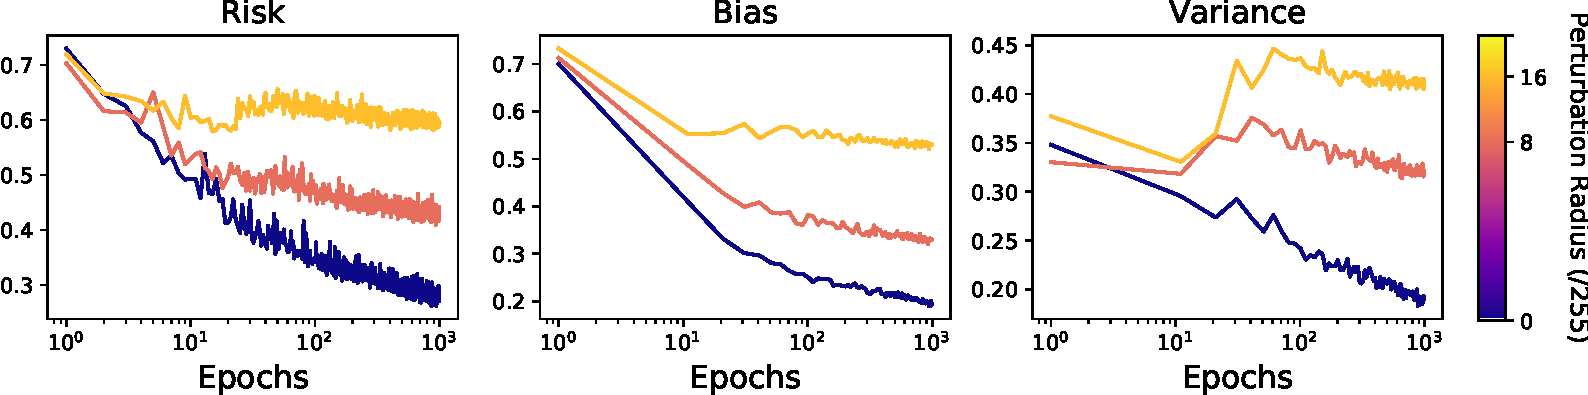
\includegraphics[width=0.95\textwidth]{figures/reason-variance.pdf}
%   \caption{``Risk'' (Average test error over independent training subsets) obtained when training on an adversarially augmented dataset, as well as the ``Bias'' and ``Variance'' following a bias-variance decomposition of the 0-1 loss. Detailed experiment settings can be found in Appendix~\ref{sect: exp-ad-augment}.
%   }
% \label{fig:dependence-variance}
% \end{figure*}




% Finally, we note that our above analyses echo the existing works. 
% Since implicit label noise modulates the double descent, and by Theorem~\ref{theo:label-noise-perturbation} it depends on the perturbation radius and data quality, the double descent in adversarial training should strongly correlate with the perturbation radius and data quality. Indeed, it has been observed respectively that small perturbation radius will not induce robust overfitting~\citep{Dong2021ExploringMI}, and high-quality data will not induce robust overfitting~\citep{Dong2021DataPF}.
% for small perturbation radius and high-quality dataset, the double descent may not be observed in adversarial training, which echos the recent empirical observation made in \citet{Dong2021ExploringMI} and \citet{Dong2021DataPF} respectively.